\documentclass[tikz,border=8pt]{standalone}
\usepackage{times}
\usepackage{amsmath}
\usetikzlibrary{arrows.meta,calc}
\begin{document}
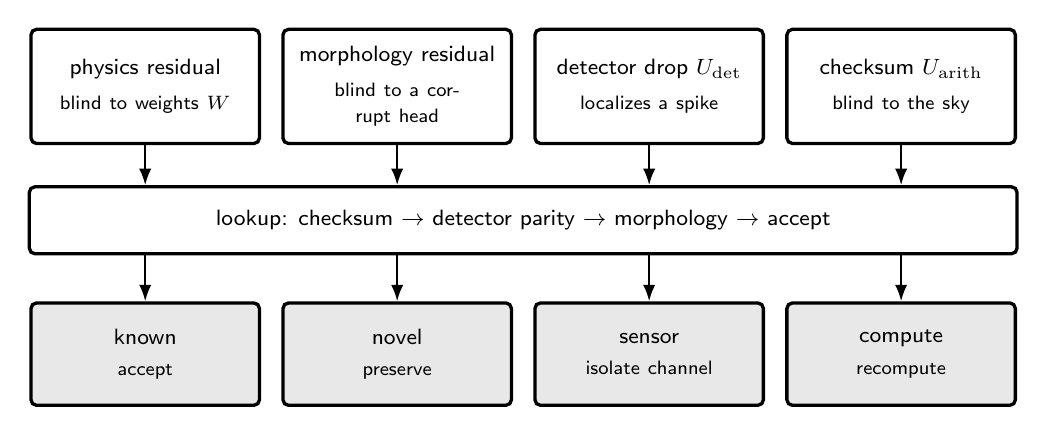
\begin{tikzpicture}[
  font=\sffamily\footnotesize,
  res/.style={
    draw, very thick, rounded corners=2pt, align=center,
    inner sep=5pt, minimum height=1.45cm, text width=2.55cm,
  },
  cause/.style={
    res, fill=black!9, minimum height=1.3cm,
  },
  look/.style={
    draw, very thick, rounded corners=2pt, align=center,
    inner xsep=6pt, inner ysep=7pt, minimum height=0.85cm,
  },
  arr/.style={-{Latex[length=2.1mm]}, thick},
]
\def\dx{3.2}
\node[res] (phys)  at (0,    3.55) {physics residual\\[3pt]{\scriptsize blind to weights $W$}};
\node[res] (morph) at (\dx,  3.55) {morphology residual\\[3pt]{\scriptsize blind to a corrupt head}};
\node[res] (det)   at (2*\dx,3.55) {detector drop $U_{\mathrm{det}}$\\[3pt]{\scriptsize localizes a spike}};
\node[res] (arith) at (3*\dx,3.55) {checksum $U_{\mathrm{arith}}$\\[3pt]{\scriptsize blind to the sky}};

\path let \p1=(phys.west), \p2=(arith.east) in
  node[look, minimum width=\x2-\x1] (lookup) at ({(\x1+\x2)/2}, 1.85)
    {lookup: checksum $\to$ detector parity $\to$ morphology $\to$ accept};

\node[cause] (k) at (0,    0.15) {known\\[2pt]{\scriptsize accept}};
\node[cause] (n) at (\dx,  0.15) {novel\\[2pt]{\scriptsize preserve}};
\node[cause] (s) at (2*\dx,0.15) {sensor\\[2pt]{\scriptsize isolate channel}};
\node[cause] (c) at (3*\dx,0.15) {compute\\[2pt]{\scriptsize recompute}};

\foreach \src in {phys,morph,det,arith}
  \draw[arr] (\src.south) -- (\src.south |- lookup.north);
\foreach \dst in {k,n,s,c}
  \draw[arr] (\dst.north |- lookup.south) -- (\dst.north);
\end{tikzpicture}
\end{document}
